\section{Core Concepts of Machine Learning}
Machine learning and natural language processing are important components laying at the foundation of this thesis. Therefore, the current chapter provides an overview of some of the relevant fundamental concepts, required for understanding the thesis further on.

\subsection{Introduction}

Artificial intelligence (AI), originally coined as a term and founded as an academic discipline in the 1950s \cite{a5}, has become a buzzword not only in the domain of computer science, but also in the popular culture. The growth in popularity and general interest is owed to the accelerated technological advancements and exponential increase in the volumes of data, which fueled the progression of AI from mostly bare theory to a gradual actuality.

There is no singular universally accepted definition for artificial intelligence. This term generated a considerable amount of differences and confusion among specialists\cite{a6}. There are numerous proposed definitions, but one that encapsulates to a certain extent a common essence encountered in a fair part of them could be formulated as follows:

\begin{definition}
  Artificial intelligence is a branch of computer science, concerned with developing computer programs that approach problems emulating the human model of thinking and its typical processes, such as learning, reasoning and self-correction.
\end{definition}

Another term coined in the 1950s is "machine learning". Machine learning is a subfield of artificial intelligence, based on the idea that computers can be programmed to "learn" from data and tackle tasks with minimal human intervention. A definition for this field of study, based on Tom Mitchell's proposal \cite{b1}, is the following one:

\begin{definition}
  Machine learning studies the capability of a computer program to learn from experience E with respect to some task T and some performance measure P, improving with experience E its performance on the task T, measured by P.
\end{definition}

This definition is a more mathematical one, operating with three variables:
\begin{enumerate}
  \item E (experience) stands for the dataset collected for the learning process, which is leveraged for extracting a general formula from a set of particular examples.
  \item T (task) represents the problem which is desired to be solved via a machine learning algorithm.
  \item P (performance measure) refers to a set of metrics applied on the machine learning model to mathematically quantify its performance.    
\end{enumerate}

Machine learning is a novel field which has been successfully implemented and notably pushed the boundaries in many real applications, including pattern recognition, speech recognition, audio processing, natural language processing (e.g. language translation, search results, smart assistants, text analysis) and computer vision (e.g. object detection, image classification, segmentation).

Out of these, natural language processing has probably the most applications in the area of fake news detection, the subject of this thesis.

\begin{definition}
  Natural language processing (NLP) is a field of study at the intersection of artificial intelligence and linguistics, which is comprised of a range of computational techniques for analyzing and representing human language \cite{a8}.
\end{definition}


\begin{figure}[H]
  \centering
  \fbox{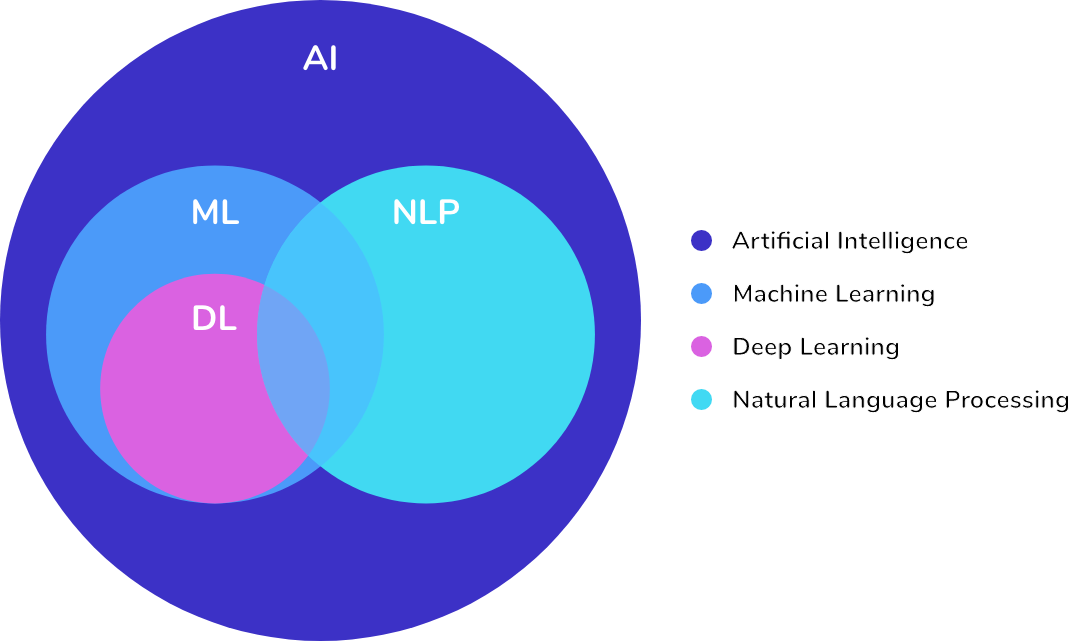
\includegraphics[width=0.9\textwidth,keepaspectratio]{images/ai-dl-ml-nlp-diagram.png}}
  \caption{Relation between NLP and Machine Learning.}
\end{figure}

\subsection{More on Machine Learning}
\subsubsection{Core Concepts of Supervised Learning}
Machine learning algorithms can be divided into three categories: \textbf{supervised learning}, \textbf{unsupervised learning} and \textbf{reinforcement learning}. Supervised learning algorithms are trained on a set of input-output pairs, with the aim of creating a mathematical model to map any general input to an output. Conversely, unsupervised learning techniques deal with unlabelled data from which patterns are derived, through various clustering and association algorithms. Lastly, reinforcement learning alg involves algorithms learning by being rewarded for desired behaviors and punished for undesired ones. 

In the context of fake news detection, the majority of research revolves around supervised learning algorithms, hence that is what this thesis will further focus upon.

Supervised learning operates with annotated (labeled) datasets during the training and testing process. Every element from the training dataset is called a feature vector, in which each dimension (i.e. feature) characterizes the input data from a certain aspect. The goal is to learn the correlation between the set of features and the labels for every training example, so that through generalization, the label of a potentially unmet input can be predicted. This process of identifying correlations, anomalies and patterns within a dataset is known as \textbf{data mining}. 

There are generally no perfect models that can generate the correct output with 100\% accuracy for all of the inputs. The discrepancies between the ground truth labels and the actual predictions of the model can be expressed by a \textbf{loss function}. Thereby, the purpose of the supervised learning algorithm can also be understood as the minimization of the loss function, which translates into the maximization of the accuracy and other performance metrics of the model.

Supervised learning algorithms can be split into two types: \textbf{classifications} and \textbf{regressions}. Both algorithms are used for making predictions, but they differ primarily in the type of the output produced. For a given input, classification algorithms predict discrete values, called classes or categories, from a finite set of values, to which the feature vectors are considered to belong. Contrarily, regression algorithms predict continuous values (integer or floating point values), which usually denote either quantities or sizes. For instance, let us consider weather prediction based on certain parameters, such as: humidity, temperature or atmospheric pressure. This task could be approached in two ways: predict if the weather is hot or cold (binary classification) or predict a precise value for the temperature, such as 24 degrees Celsius (regression).

As for fake news detection, in order to determine whether an article is fake or real, a classification algorithm is most suitable. The algorithms employed within this project are probabilistic classifiers, which are not only able to make a categorical prediction (i.e. fake or real), but they can also compute the probability distribution of a news article over the set of classes. Probabilities are more revealing than mere binary values, because they measure the confidence with which the classifier predicts a certain class.

Within this project, the following classification algorithms were used for the problem of fake news detection: \textbf{Support Vector Machine}, \textbf{Decision Tree}, \textbf{Logistic Regression}, \textbf{K-nearest Neighbors}. 

\subsubsection{K-nearest Neighbors}
K-nearest Neighbors (KNN) is one of the simplest machine learning supervised algorithms, which is also known to be quite versatile and well-performing. It functions on the principle of proximity relative to the previous training examples. It can be used as a regression algorithm, but it is most encountered in classification problems. KNN is \textbf{non-parametric} and \textbf{lazy-learning} or \textbf{slow-learning}, the two primary properties of KNN. 

By non-parametric, it is meant that the classifier does not make any prior strong assumptions about the underlying structure of the data by deciding beforehand the number of parameters of the mapping function which the algorithm models during training. Opposed to parametric algorithms, which can discard the training data after the model is build, KNN stores each training example as a parameter and makes all the upcoming predictions based on the k most similar training patterns performed earlier on. Practically, the sole assumption the model makes is the correlation or similarity between the feature vectors analyzed previously and the new training examples.

By lazy-learning or slow-learning, it is meant that KNN is technically not having an explicit training process and it does not learn from the training data immediately. During the training phase, the KNN algorithm simply stores in memory each of the feature vectors from the training dataset, relying on observable data similarities and distance metrics.

The KNN algorithm can be outlined by the following steps which are iteratively performed for each training or testing example:
\begin{enumerate}
  \item Locate and store the feature vector on the graph, as a data point.
  \item Calculate the distance between the current data point and the rest of the previous training examples. In order to calculate the distance, various formulas can be used, such as the Euclidean distance, the Manhattan Distance, the Minkowski distance or the cosine distance.  
  \item Consider the k nearest neighbor data point and count the frequency of each label.
  \item Assign a class label to the current data point according to the majority vote rule: the label that is in the greatest proportion present around the data point, from the k considered closes ones.
\end{enumerate}

\begin{figure}[H]
  \centering
  \fbox{\includegraphics[width=0.9\textwidth,height=\textheight,keepaspectratio]{images/knn.jpeg}}
  \caption{KNN algorithm selecting the K nearest neighbors.}
\end{figure}

The \textbf{advantages} of KNN is that it is relatively simple to implement, can learn non-linear decision boundaries, no training time, new data can be added anytime without a negative effect on the accuracy and there is only one hyperparameter to handle (i.e. k). As of \textbf{disadvantages}, does not work very efficiently on large datasets and it is sensitive to noisy data.



\subsubsection{Decision Tree}

Decision Tree is a supervised learning algorithm used for both classification and regression, having a tree-like structure, where the leaves correspond to output classes and the sub-branches represent series of decision rules, each leading finally to the prediction of an output class. The sub-branches are comprised of internal nodes, each of them containing different features of the dataset. Decision trees can be viewed as graphical representation covering all the solutions to a problem based on a specified set of conditions.

It is called a decision tree because comparable to a tree, it starts from the root node (representing the entire dataset) and expands to an increasing number of sub-branches gradually, learning from the past training examples. Each internal leaf stands for a decision rule. By decision rule, we mean a simple IF-THEN statement, consisting of a condition and a prediction. For instance, IF a person is 65 years old and is obese, THEN they have a high probability of hearth attack of diabetes.

There are two main operation performed on a decision tree, namely splitting (i.e. the operation of ramifying the root node or a decision node into two sub-branches) and pruning (i.e. the operation of compression of the size of the tree, by elimination unimportant or redundant sections of the tree). Also, by pruning one can reduce the complexity and overfitting from the tree.

A decision tree can be decomposed in the following steps:
\begin{enumerate}
  \item Initialize the tree with only the root node, which contains the whole dataset.
  \item Use an attribute selection measure to split the node into two sub-branches according to the best attribute.
  \item Create a new decision node containing the best attributed identified at the prior step.
  \item Recursively apply the first 3 steps to all the resulting subtrees.
  \item Stop the recursivity as soon as the nodes cannot be classified further anymore and regard the final nodes as leaves.
\end{enumerate}

\begin{figure}[H]
  \centering
  \fbox{\includegraphics[width=0.8\textwidth,keepaspectratio]{images/decision-tree.jpeg}}
  \caption{Small example of decision tree.}
\end{figure}

The pruning process mentioned above can be done in two ways: post-pruning (i.e. execute the pruning after the construction of the decision tree is completed, technique particularly used when the depth of the tree is large and shows signs of overfitting) or pre-prunning (i.e. execute the prunning some time before the completion of the decision tree, technique useful to prevent overfitting).

On the one hand, the upsides of decision tree include: less data preparation is needed (not critical to standardize and normalize the data), data scaling is not required and it has the ability to capture non-linear relationships. On the other hand, the downsides are that decision tree generally require more computational resources and execution time

\subsubsection{Logistic Regression}
Logistic regression is a supervised machine learning algorithm which is used for classifications and involves drawing a hypothesis function which best fits the categories/classes of a dataset. 

Opposed to the linear regression, where the aim is to find a linear function, logistic regression looks for other types of function, such as the commonly utilized sigmoid/logistic function. The sigmoid function is a S-shaped curve, useful for binary classification tasks, given that the domain of the function can be the whole real values set and the output is either greater than and very close to 0 or less than and very close to 1. The sigmoid function "squishes" any value towards the top and bottom margins. If the output of the sigmoid function is less than 0.5, the algorithm will predict that the data point belongs to first class, otherwise that it belongs to second class. The equation of the sigmoid function is the following one:

While in linear regression algorithms, adjusting the linear function is done by minimizing the sum of the distances between each data point to the line (i.e. the least squares method), in logistic regression the maximum likelihood estimation is used instead. The maximum likelihood estimation method attempts to maximize the conditional probability of observing the data X given a specific probability distribution and its parameters theta \cite{log_reg}.

\begin{figure}[H]
  \centering
  \fbox{\includegraphics[width=0.7\textwidth,keepaspectratio]{images/lr-sigmoid.jpeg}}
  \caption{Logistic regression sigmoid function.}
\end{figure}

The advantages of this algorithm include: efficient training process, easy and intuitive implementation, ability to easily extend to multiple classes. Conversely, there is also one major disadvantage: the constraint of linear boundaries.

\subsubsection{Support Vector Machine}
Support Vector Machine is another popular supervised learning algorithms, that is often preferred for the high accuracy along with low computation power. The main idea of the algorithm is to search for a hyperplane which separates the data points into the possible output classes.

From all the possible hyperplanes meeting this requirement, the algorithm has to specifically select that which is furthest from the data points of each category. Maximizing the margin between the hyperplane and the data points results in a more solid decision boundary between the classes, making the predictions more confident and reliable. If the hyperplane is discrepantly closer to the data points of a certain class and further from another class, then the observation located in the close proximity of the hyperplane could be classified in the group which is considerably further from.

\begin{figure}[H]
  \centering
  \fbox{\includegraphics[width=0.8\textwidth,keepaspectratio]{images/svm-hyperplane.jpeg}}
  \caption{Hyperplane too close to one of the classes.}
\end{figure}

The name of "Support Vector Machine" reveals the essential elements that the algorithms is based upon: support vectors (i.e. data points that are closest to the hyperplane and which influence the position and orientation of the hyperplane).

\begin{figure}[H]
  \centering
  \fbox{\includegraphics[width=0.7\textwidth,keepaspectratio]{images/svm.jpeg}}
  \caption{Support Vector Machine optimal hyperplane.}
\end{figure}
